%%%%%%%%%%%%%%%%%%%%%%%%%%%%%%%
\chapter{Element Operators}

Currently element operators over a series of blocks of elements on
different types of architecture and devices are to be found in the
Operator library. These operators work on a block of elements with
similar expansion bases, quadrature and are either \texttt{regular} or
\texttt{deformed} geometries.

Currently we have implementation for the operators

    \begin {table}[htbp!]
    \begin{center}
    \scalebox{0.9}[1.]{
    \begin{tabular}{ |l | l| l|}
      \hline      
      \textbf{Description} & \textbf{Function short name} & \textbf{ Mathematical formd} \\  
      \hline
Backward transform $\hat{u}_{pq}$ to $u(\beta_1, \eta_2)$ &  \texttt{BwdTrans}  &  $u(\eta_{1i}, \eta_{2j}) = \sum_{pq} \phi_{pq}(\eta_{1i}, \eta_{2j}) \hat{u}_{pq}$\\
      \hline
Inner Product of $f$ with respect to  &  \texttt{IPRoductWRTBase}  &  $I_{pq} = (\phi_{pq}, f)$\\
the basis $\phi_{pq}$ &   & \\
      \hline
Inner Product of a vector  ${\bf f}$ with &  \texttt{IPRoductWRTDerivBase}  &  $I_{pq} = (\nabla \phi_{pq}, {\bf f})$\\
respect to the grad of the basis $\phi_{pq}$ & & \\
      \hline
Derivative of $u$ in physical & \texttt{PhysDeriv} & ${\bf d} = \nabla u$  \\
or quadrature space & & \\
      \hline
Mass matrix operator on $u = \sum_{rs} \phi_{rs} \hat{u}_{rs}$ & \texttt{Mass} & $ I_{pq}  = (\phi_{pq}, u) = (\phi_{pq}, \sum_{rs} \phi_{rs} \hat{u}_{rs})$  \\
      \hline
Weak Helmholtz operator on $u$& \texttt{Helmholtz} & $ I_{pq}  = (\nabla \phi_{pq}, \nabla u) + \lambda (\phi_{pq}, u)$  \\
      \hline
      Interpolate $u^P(\eta_1,\eta_2)$  to a 1D scaled  & \texttt{PhysInterp1DScaled} & 
    $u(\eta^{\sigma P}_{1i}, \eta^{\sigma P}_{2j}) = $\\
factor, $\sigma$, number of quad. points && \hspace{12pt} $\sum_{pq} h^P_{p}(\eta^{\sigma P}_{1i}) h^P_{q}(\eta^{\sigma P}_{2i}) u^P_{pq}$  \\
      \hline
    \end{tabular}
    }
    \end{center}
    \caption {Table of element operations and their mathematical form} \label{tab:elmtops} 
    \end{table}



\section{File structure}

Within the \texttt{ElmtOps} directory there are a series of
sub-directories which Function short name from table
\ref{tab:elmtops}. In configuration using CMake the filename is used
to identify which operators are available for compilation and so
adding a new elemental operator \texttt{MyOps} would require a new
directory of the same name.

Also wihtin the \texttt{ElmtOps} directory you will find a series of
.hpp files with the naming format
\texttt{Operator\{FunctionShortName\}.hpp} where the
\texttt{FunctionShortName} again refers to that provided in table
\ref{tab:elmtops}. These files contain the parent class definition
typically names \texttt{Operator\{FunctionShortName\}}. As indicated by
figure \ref{fig:elmtops} from doxygen all of these classes inherit
public methods from the \texttt{OperatorElmt} class which is defined
in \texttt{OperatorElmt.hpp} which also inherits from the
\texttt{Operator} class defined in the file
\texttt{Common/OPerator.hpp} file in the main director of the Operator
library.


\begin{figure}[htbp]
  \centering
  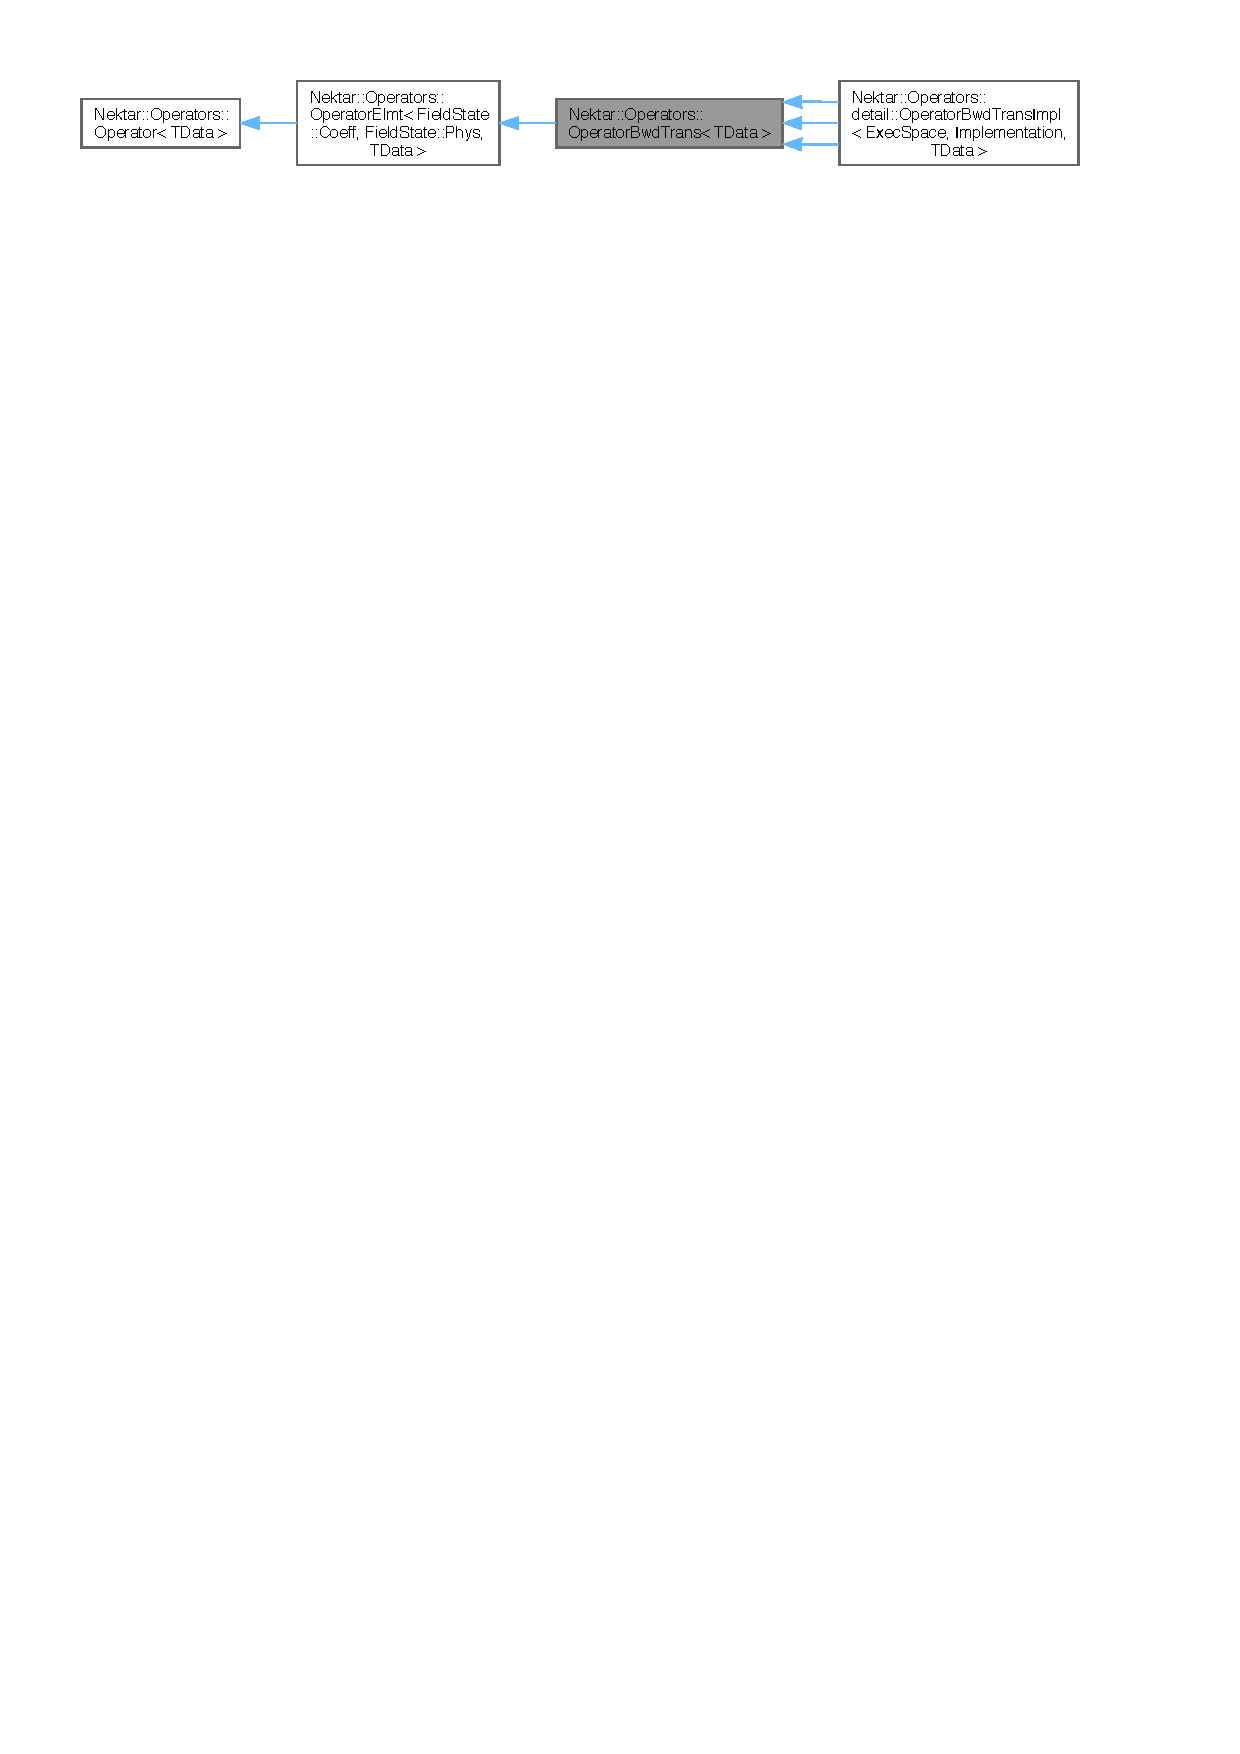
\includegraphics[width=1.0\textwidth]{img/operatorBwdTransInheritGraph.pdf}
  \caption{inheritance of element operator class}
  \label{fig:elmtops}
\end{figure}

As indicated in figure \ref{fig:elmtops}, three classes also inherit
from the class \texttt{OperatorBwdTrans} and this relates to a CPU/AVX
sum factorisation implementation, a Standard matrix CPU implementation
and a GPU implementation with variants for Cuda, Kokkos and SYCL. We
will next discuss this formatting for each of these implementations.

\subsection{Sum factorisation Matrix operators on CPUs with and without AVX}

Sum factorisation utilises the tensor product nature of the expansions
and permits a series of one-dimensional type operations. Using the
SIMD library approach discussed in section \ref{sec:simdlib} we are
able to reuse the same code for both a scalar and vector approach
which can accomdate the sum factorisation over each elements at a time
in the case of a scalar approach or multiple elements in the case of
an AVX acceleration where the number of elements depends on the AVX
instruction set. More details of the AVX implementation can be found
in reference \cite{moxey2020efficient}.


The derived implementation class should be placed in a file named

\inlsh{\{FunctionShortName\}SerialAvXSumFac.hpp}

\noindent where as previously
discussed \texttt{FunctionSHortName} is proivded in table
\ref{tab:elmtops} for each operator.

In this file the size of the SIMD type is selected from definining \texttt{simd\_t}, i.e.

\begin{lstlisting}[style=C++Style]
template <typename ExecSpace, typename Implementation, typename TData>
class OperatorBwdTransImpl : public OperatorBwdTrans<TData>
{
    using simd_t =
        typename simd_type_if<std::is_same_v<ExecSpace, NektarSpaces::AVX>,
        TData>::type;
\end{lstlisting}

where \texttt{simd\_type\_if} is defind in \texttt{Common/Operator.hpp} as 


\begin{lstlisting}[style=C++Style]
template <bool B, typename TData> struct simd_type_if
{
    typedef tinysimd::scalarT<TData> type;
};

template <typename TData> struct simd_type_if<true, TData>
{
    typedef tinysimd::simd<TData> type;
};
\end{lstlisting}

Therefore by default \texttt{simd\_t} is defined as
\texttt{tinysimd::scalarT<TData>} but if \texttt{ExexSpace} is
\texttt{NektarSpaces::AVX} then it is set to
\texttt{tinysimd::simd<TData> }.

This class holds appropriate intialisation such as refernece to the 1D
Expansion basis and also has the specific implementation of the
\texttt{apply()} method. This method has a generic form which just
loops over the blocks in the form:

\begin{lstlisting}[style=C++Style]
    void apply(Field<TData, FieldState::Coeff> &in,
               Field<TData, FieldState::Phys> &out) override
    {
        // Initialize index.
        size_t exp_idx = 0;

        for (size_t blk = 0; blk < in.GetBlocks().size(); ++blk)
        {
            m_expPtr = this->m_expansionList->GetExp(exp_idx);

            // Block dependent.
            auto &inblock  = in.GetBlocks()[blk];
            auto &outblock = out.GetBlocks()[blk];

            this->BlockOperator(inblock, outblock);

            // Increment index for next element type.
            exp_idx += inblock.GetNumElements();
        }
    }
\end{lstlisting}

The method \texttt{BlockOperator()} then primarily contains a switch statement which calls shape dependent block operators, i.e.

\begin{lstlisting}[style=C++Style]
        switch (shapeType)
        {
            // Segment
            case LibUtilities::Seg:
            {
                SegBlock(inblock, outblock);
                break;
            }
            // Quads
            case LibUtilities::Quad:
            {
                QuadBlock(inblock, outblock);
                break;
            }
            // Triangles
            case LibUtilities::Tri:
            {
                TriBlock(inblock, outblock);
                break;
            }
            ....
            }
\end{lstlisting}

These shape block operators are then defined in separate files which
are auto generated using the Cmake \texttt{Configure\_file()} method.
This file is named

\inlsh{\{FunctionShortName\}SerialAVXSumFacBlockOp.cpp.in}

\noindent and includes another auto generated file of the form
\texttt{BlockOpSwitchCodeShape.h} where \texttt{Shape} is
\texttt{Seg,Quad,Tri,Hex,Prism,Pyr,Tet}. In these file we use Boost
preprocessing to generate a switch statement to call templated
versions of the methods \texttt{Operator1D(), Operator2D()} or
\texttt{Operator3D()} which are defined in the original file

\inlsh{\{FunctionShortName\}SerialAvXSumFac.hpp}.

\noindent The switch statement runs over all polynomial or qudarture
orders that are defined by the Cmake defined options
\texttt{NEKTAR\_SWITCH\_MIN} and \texttt{NEKTAR\_SWITCH\_MAX} and
assume that each polynomial order is the same and that the standard
quadrature orders are applied for each shape. For operators involving
both polynomial and quadrature orders the quadrature order runs from
the polynomial order to twice the polynomial order. The boost
preprocessing code look in the files similar to
\texttt{Common/BlockOpSwitchCode.h.in}.  This rather convoluted file
structure helps abstract the boost prepropcessing codes and also
speeds up the compilation which otherwise is rather slow due the large
switch statement that are generated to call the templated code.

Finally the methods \texttt{Operator1D(), Operator2D()} or
\texttt{Operator3D()} are defined in a templated and non-templated method
for use in the switch statements and to also have a default method for
cases whcih are not covered in the templated parameters in the switch
statement. These methods also call kernel functions for each method
that contain the primary code for each method and can be found in the
files

\inlsh{\{FunctionShortName\}SerialAVXSumFacKernels.hpp}

\noindent and also in the \texttt{StdRegions/Operators/} directory.


\subsection{Standard Matrix operators on CPUs}

The idea behind the standard matrix approach is to identify, where
possible, a matrix operator in standard region which can be used on a
whole block of elements. More details on this approach can be found in
\cite{Collections}. This approach is currently only setup for serial
operations on a CPU.

If it is possible to define a standard matrix approach the derived
implementation class can be  defined in a file named

\inlsh{\{FunctionShortName\}SerialStdMat.hpp}. 

\noindent where as previously \texttt{FunctionShortName} is taken from
table \ref{tab:elmtops}. In constructing the method a series of
standard matrices are setup for each elemental block. These matrices
are of dimension of the total number of quadrature points or
expansion modes and so can become quite large for higher
polynomial orders.

The \texttt{apply()} method once again looks over each series of
blocks and essentially makes calls to a large blas3 DGEMM()
matrix-matrix calls invovling the quadrature points or epxansion modes
and the number of elements in a block.

\subsection{GPU using Kokkos, SYCL and native coding}

The file and class structure of the GPU devices is anaologous to the
Serial/AVX structure. The derived implementation class is defined
in the file

\inlsh{\{FunctionShortName\}DeviceSumFac.hpp}. 

\noindent where as previously \texttt{FunctionShortName} is taken from
table \ref{tab:elmtops}. This file contains the required
initialisation for a given operator and the \texttt{apply()} method
loops over the blocks of elements and evaluate the operation in an
identical manner to the previous implementations. As previously
outlined the \texttt{apply()} method calls a \texttt{BlockOperator()}
method which contains a switch statement to call a shape dependent
method, i.e. \texttt{TriBlock(), QuadBlock(), HexBlock(), ...} and as
previously these shape dependent methods are auto generated in
different files to help with compilation speed and to wrap the primary
method in a boost prepocessing auto generated swith statement to allow
for the possibility of a templated veresion of the operator to be
called if the quadrature and polynomial order of the elements in a
block are of equal order polynomial order in all dimensions and have
the standard quadrature points used in equi-ordered polynomial
expansions. The details for the auto generated shape dependent block
operator code can be found in the files

\inlsh{\{FunctionShortName\}DeviceSumFacBlockOp.cpp.in}

and 

\inlsh{\{FunctionShortName\}DeviceSumFacQPBlockOp.cpp.in}

\noindent where \texttt{QP} refers to Quadrature Point implementation
strategy outlined below. The boost preprocessing directives called
from these files can be found in the file

\texttt{Common/BlockOpSwitchCode.h.in}.

\noindent As mentioned previously the
polynomial and quadrature range of the switch is determined by the
Cmake defined parameters \texttt{NEKTAR\_SWITCH\_MIN} and
\texttt{NEKTAR\_SWITCH\_MAX}.

The shape based block operator methods call the methods
\texttt{Operator1D(), Operator2D()} or \texttt{Operator3D()} which are
defined in the original file

\inlsh{\{FunctionShortName\}DeviceSumFac.hpp}. 

\noindent where there is either a templated verion of the method with
polynomial and quadrature order as template values or non-templated
method which acts as a default for the switch statements.

THe method \texttt{Operator1D(), Operator2D()} or
\texttt{Operator3D()} contain code to check the input and output
arrays for the correct interlacing, initialise work space as well as
access the required data for he kernel operators such as the basis
array or 1D derivaitve matrices. This data is then passed to a kernel
method which is contained in

\inlsh{\{FunctionShortName\}DeviceSumFacKernels.hpp}.

This file then includes method specific kernels for the Cuda, Kokkos
or SYCL implementations. The inclusion of the Cuda, Kokkos and SYCL
code depends on the CMAKE options \texttt{NEKTAR\_ENABLE\_CUDA},
\texttt{NEKTAR\_ENABLE\_KOKKOS} and \texttt{NEKTAR\_ENABLE\_SYCL} and
the related kernel code can be found in the files:

\inlsh{\{FunctionShortName\}CUDASumFacKernels.cuh},\\
\inlsh{\{FunctionShortName\}KokkosSumFacKernels.cuh},\\
\inlsh{\{FunctionShortName\}SYCLSumFacKernels.cuh}.

Finally we have two implementations of the sum factorisation kernels,
denoted \texttt{SumFac} and \texttt{SumFacQP}. The first
\texttt{SumFac} approach maps each elemental operation to a CUDA-thread
for a completely vectorised kernel, whilst in the second
\texttt{SumFacQP} approach, each element is mapped to a CUDA-block for
nested parallelism and requires an indexing to each quadrature point
(\texttt{QP}) or modal expansion. Results from \cite{GPU_Vector} show
that the first approach is beneficial for elements with low polynomial
order, whereas the second approach is beneficial for elements of
higher order.

